\section{Star Anise}
\label{sec:star_anise}

\begin{spice}\label{spice:star anise}
\textsc{Star anise} \hfill \href{https://powo.science.kew.org/taxon/554553-1}{POWO} \\
\textbf{English:} \textit{star anise}. 
\textbf{Arabic:} {\arabicfont{يانسون نجمي}} \textit{yānsūn najmī} [star anise]. 
\textbf{Chinese:} {\traditionalchinesefont{八角}} \textit{bājiǎo} [octagon]. 
\textbf{Hungarian:} \textit{csillagánizs} [star-anise].  \\
\noindent{\color{black}\rule[0.5ex]{\linewidth}{.5pt}}
\begin{tabular}{@{}p{0.25\linewidth}@{}p{0.75\linewidth}@{}}
Plant species: & \taxonn{Illicium verum}{Hook.f.} \\
Family: & \textit{Schisandraceae} \\
part used: & pericarp \\
Region of origin: & SE. China; Vietnam \\
Cultivated in: & China; Laos; Vietnam; Korea; Japan; Taiwan; Hainan; Philippines (POWO) \\
Color: & orange brown \\
\end{tabular}
\end{spice}

\begin{figure}[!ht]
	\vspace{-4ex}
	\centering
	\subfloat[\centering]{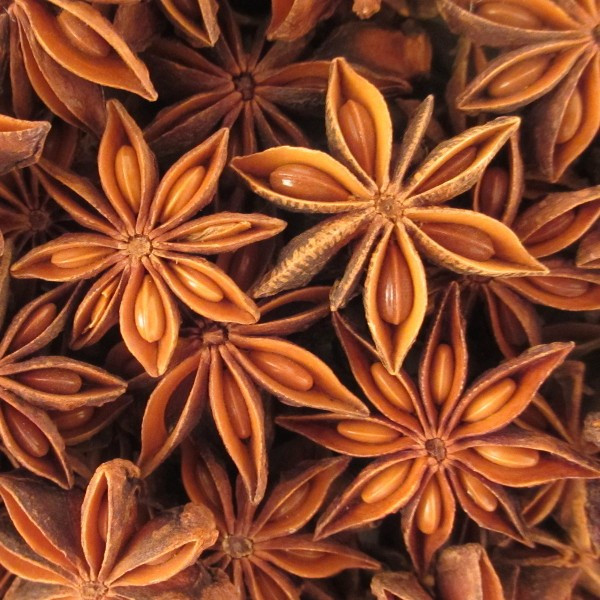
\includegraphics[width=0.3\linewidth]{imgs/spices/star_anise-1.jpg}}
	\hfill
	\subfloat[\centering]{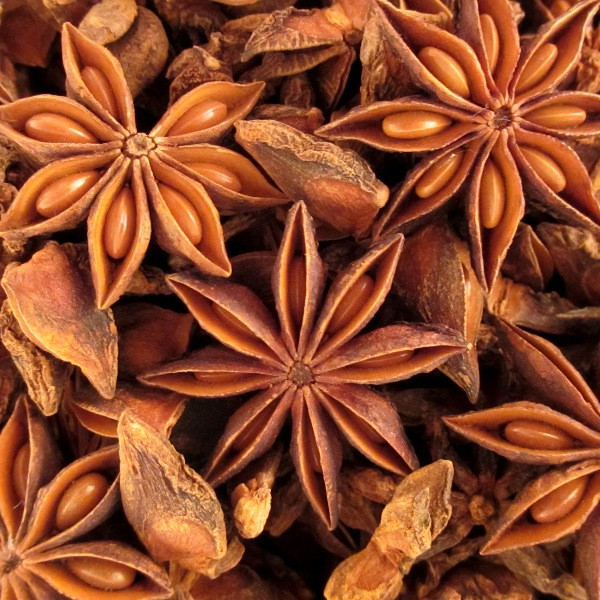
\includegraphics[width=0.3\linewidth]{imgs/spices/star_anise-2.jpg}}
	\hfill
	\subfloat[\centering]{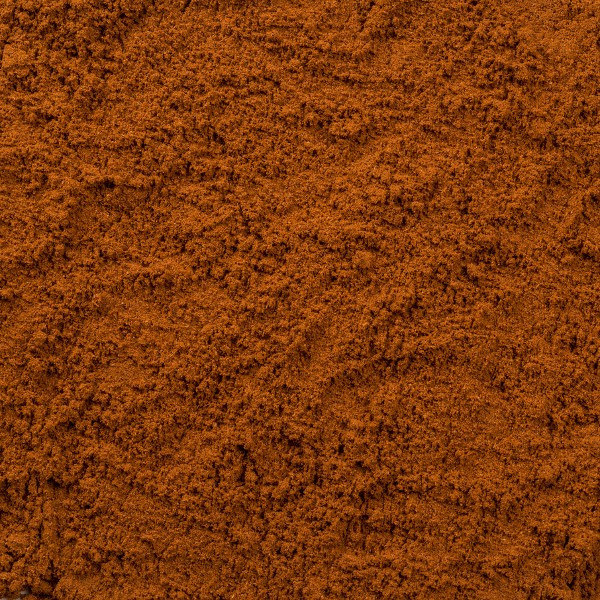
\includegraphics[width=0.3\linewidth]{imgs/spices/star_anise-3.jpg}}
	\caption{Star Anise \taxon{Ilicium verum}. Credit: Aromatiques.}
	\label{fig:star_anise_imgs}
\end{figure}

Star anise is a spice consisting of the dried fruits of the tree \textit{Illicium verum}. 

% DAVIDSON:
% a spice consisting of the small, star-shaped, dried fruits of Illicium verum, a slender evergreen tree of the family Illicaceae related to Magnoliacea. This is not known in the wild state, but is assumed to be indigenous to China. It is not a relation of anise, but shares with it the same essential oil, anethole, which is used for flavouring some drinks and confectionery; star anise is the principal commercial source of anethole.

% The appearance of the fruit is remarkable. Eight (rarely, 9 or 10) carpels attached to a central column produce the starlike shape. These carpels, which can be over 15 mm (0.25") long and are often irregularly developed, are dark reddish-brown in colour; each normally contains one hard light brown seed.

% Cultivation, which is not easy, is almost entirely confined to S. China and parts of SE Asia.

% Star anise is one of the ingredients of (Chinese) five spice. Jill Norman (1990) observes that it occurs in some western recipes for syrups and jams in the 17th century; and that some western chefs now use it in, for example, fish stews. In China it has been associated with pork and poultry.

\subsection{The Botany, Origins, and Cultivation of Star Anise}

\subsection{The History of Star Anise}

Star anise has been known in China as a spice and medicine for over 3,000 years. When in 970 AD, the southern states lost a cruel and merciless war with the Chinese emperor, they had to pay war reparations in star anise. The English pirate Sir Thomas Cavendish brought star anise to Europe from the Philippines in 1588. It began appearing in European kitchens during the 17th century as an aromatic agent added to tea in the Russian Czar's court. It was not used in Germany until the end of the 18th century. The genus name Illicium comes from the Latin illicere, meaning lure or attract.

% http://spices.biodiversityexhibition.com/en/card/star-anise

\subsection{The Names of Star Anise}

\subsubsection{English}

% https://en.wiktionary.org/wiki/%D8%A8%D8%A7%D8%AF%DB%8C%D8%A7%D9%86

\begin{etymology}\label{ety:star anise}
\textbf{English} \textit{star anise} `star anise'\footnote{}
\end{etymology}
\begin{etymology}\label{ety:badian}
\textbf{English} \textit{badian} `star anise', 1693
< \textbf{French} \textit{badiane} `star anise', 1681
< \textbf{Persian} {بادیان} \textit{bādyān} `fennel; anise'\footnote{\textcite{oed}; \textcite{tlfi}; \textcites[140]{steingass_comprehensive_1892}[197]{hayyim_new_1934}}
\end{etymology}

\begin{table}[!ht]
\centering
\begin{tabularx}{\textwidth}{@{}l>{\itshape \small}lL>{\small}l@{}}
\toprule
\textbf{\#} & \multicolumn{1}{l}{\textbf{Species}} & \multicolumn{1}{l}{\textbf{Name}} & \multicolumn{1}{l}{\textbf{Source}} \\
\midrule
1	& Illicium verum	& badian	& \textcite{oed} \\
2	& Illicium verum	& Chinese anise	& \textcite{van_wyk_culinary_2014} \\
3	& Illicium verum	& Chinese fennel	&  \\
4	& Illicium verum	& Chinese star anise	& \textcite{van_wyk_culinary_2014} \\
5	& Illicium verum	& Siberian anise	&  \\
\textbf{6}	& \textbf{Illicium verum}	& \textbf{star anise}	& \textbf{\textcite{van_wyk_culinary_2014}} \\
\bottomrule
\end{tabularx}
\caption{Various names for star anise in English.}
\label{table:names_star_anise_en}
\end{table}



\subsubsection{Arabic}

\begin{table}[!ht]
\centering
\begin{tabularx}{\textwidth}{@{}l>{\itshape \small}lr>{\itshape}lL>{\small}l@{}}
\toprule
\textbf{\#} & \multicolumn{1}{l}{\textbf{Species}} & \multicolumn{1}{l}{\textbf{Name}} & \multicolumn{1}{l}{\textbf{Tr.}} & \multicolumn{1}{l}{\textbf{Gloss}} & \multicolumn{1}{l}{\textbf{Source}} \\
\midrule
1	& Illicium verum	& ليسوم حقيقي	& laysūm ḥaqīqī	& true illicium	& \textcite{wikipedoa} \\
2	& Illicium verum	& نجمة اليانسون الصينية	& najmat al-yānsūn al-ṣīniyya	& Chinese star anise	&  \\
\textbf{3}	& \textbf{Illicium verum}	& \textbf{يانسون نجمي}	& \textbf{yānsūn najmī}	& \textbf{star anise}	& \textbf{} \\
\bottomrule
\end{tabularx}
\caption{Various names for star anise in Arabic.}
\label{table:names_star anise_ar}
\end{table}



\subsubsection{Chinese}

\begin{table}[!ht]
\centering
\begin{tabularx}{\textwidth}{@{}l>{\itshape \small}ll>{\itshape}lL>{\small}l@{}}
\toprule
\textbf{\#} & \multicolumn{1}{l}{\textbf{Species}} & \multicolumn{1}{l}{\textbf{Name}} & \multicolumn{1}{l}{\textbf{Tr.}} & \multicolumn{1}{l}{\textbf{Gloss}} & \multicolumn{1}{l}{\textbf{Source}} \\
\midrule
1	& Illicium verum	& \traditionalchinesefont{舶茴香}	& bóhuíxiāng	& ship-hui-spice	&  \\
2	& Illicium verum	& \traditionalchinesefont{八角}	& bājiǎo	& eight-horns/octagon	& \textcite{hu_food_2005} \\
\textbf{3}	& \textbf{Illicium verum}	& \textbf{\traditionalchinesefont{八角茴香}}	& \textbf{bājiǎohuíxiāng}	& \textbf{eight-horned-hui-spice}	& \textbf{\textcite{hu_food_2005}} \\
4	& Illicium verum	& \traditionalchinesefont{大料}	& dàliào	& big-ingredient	& \textcite{defrancis_abc_2003} \\
5	& Illicium verum	& \traditionalchinesefont{大茴香}	& dà​huíxiāng	& big-hui-spice	& \textcite{hu_food_2005} \\
\bottomrule
\end{tabularx}
\caption{Various names for star anise in Chinese.}
\label{table:names_star_anise_zh}
\end{table}



\subsubsection{Summary}

\begin{table}[!ht]
\centering
\begin{tabularx}{\textwidth}{@{}ll>{\itshape}lLl>{\small}l@{}}
\toprule
\textbf{\#} & \textbf{Language} & \multicolumn{1}{l}{\textbf{Term}} & \textbf{Gloss} & \textbf{Loan} & \multicolumn{1}{l}{\textbf{Source}} \\
\midrule
1	& English	& badian	& 	& yes	& \textcite{oed} \\
2	& English	& Chinese anise	& 	& no	& \textcite{oed} \\
3	& English	& star anise	& 	& no	& \textcite{oed} \\
\midrule
\midrule
1	& Chinese	& bājiǎo	& eight-horns/octagon	& no	& \textcite{defrancis_abc_2003} \\
2	& Chinese	& bājiǎohuíxiāng	& eight-horned-hui-spice	& no	& \textcite{kleeman_oxford_2010} \\
3	& Chinese	& dàliào	& big-ingredient	& no	& \textcite{defrancis_abc_2003} \\
4	& Chinese	& dà​huíxiāng	& big-hui-spice	& no	& \textcite{mdbg} \\
\bottomrule
\end{tabularx}
\caption{Conventionalized names for star anise in English, Arabic, and Chinese, found in dictionaries.}
\label{table:names_star_anise}
\end{table}






% Mandarin: 八角 (zh) (bājiǎo), 八角茴香 (zh) (bājiǎohuíxiāng), 大茴香 (zh) (dàhuíxiāng)

% Illicium comes from the Latin illicio meaning "entice" or "seduce".[3]

% Verum means "true" or "genuine".[3]

% The name "badian" appears to derive, via French badiane, from the apparently descriptive Chinese name for it, 八角, pinyin: bājiǎo, lit. "eight horns". However, a derivation from the Persian بادیان bādiyān, "fennel", exists, with the Oxford English Dictionary indicating that its origin before that is unknown.[4] 

\textit{Da liao} `major spices' refers to a combination of spices where star anise is the main ingredient, it is used to season meat. What da liao is made up of varies from place to place, but the presence of star anise is constant \parencite[152]{hu_food_2005}.  










% Gabor:

% My search did not (as expected) turn up any confirmed words for star anise in pre-Qin Chinese. However, I did find this in Zhou Li (rituals):

% 翦氏掌除蠹物。以攻禜攻之。以莽草熏之

% Where this refers to a kind of plant that can be burned to smoke out and/or kill bookworms, termites etc. Interestingly, this has been widely cited as referring to the Japanese star anise and indeed the term 莽(草) has been uses consistently in Benchao and Song-Ming-Qing text to refer to the Japanese star anise in contrast with star anise 八角

% Given the known central role star anise played in Chinese cuisine, and given the sparseness of inherited texts from nearly three thousand years, it is not unreasonable to assume one of the following scenarios

% 1. there was another word for star anise, but relevant documentation simply did not survive  

% 2.that 莽 was the form used to refer to both Chinese star anise and Japanese,  but unfortunately it did not survive.

% 3. That there was a different form, such as 茴(香), but again not text survive to today.

% Given any of the three scenarios, the likelihood that there was such as character is pretty high.   And, given the chance, I would guesstimate that it should have been  莽 to stand for all star anise-like plants.

% For the use of 大/小  to refer to unmarked/marked proper/imitator

% This is fairly well known but DING Jing's PolyU thesis (and later book published in Springer in 2019(?)) is the most comprehensive semantics of the use of opposites in Mandarin. Not similar 'unmarked' interpretation also show up in English morphosemantics in a different context (e.g.,length, width)...Even though 大/小 is typically translated as greater/lesser, it is somewhat misleading. Trandiationally, 大 is use more often, such as in almost all dynastic names,  大秦/大漢/大唐 . These are simply 秦/漢/唐 without 'lesser'-x in contrast. They are simply indicating an unmarked = 'the proper' meaning. 小登科 little_NameAnnounced is not real 登科 NameAnnounced "success in testing to be imperial official", but 'getting married'.  Modern Mandarin rarely uses this contrastive 大 to undeliner (un)markedness but uses 小, e.g.,小東京 小台北 小巨蛋 小聯合國  they typically to 'something that aspires to be x (and is not a real x). And occasionally both terms are used in contrast, such as 
% 大米 rice 小米 millet; 大年夜 new year's eve 小年夜  the night before new year's eve, 大月氏/小月氏 differentiate the Yuezhi proper (where they have their own kingdom) and 'lesser' (the remaining population that was conquered) 

% Thank you so much, this is very useful!
% Japanese star anise (Illicium anisatum) looks absolutely the same as Chinese star anise (Illicium verum), but it is poisonous, and only used to make incense, indeed. And for this reason, most of modern (pharmaceutical) literature is about identification and adulteration detection. (It was banned to import to the US until 1971).
% I did not know about the 大/小 case, thank you for the explanation, it explains a lot.




% nd for all others.

% On a less 'relevant' issue, the issue that caught my attention with the Japanese star anise is the constant comparison with bajiao/Chinese star anise for several historical texts and in modern texts.  Given the da/xiao dichotomy, and the Chinese radical convention of grouping the 'similar but not the same' in the same category, I cannot but suspect that these two 'star anises' were assigned one identical term at sometime historically.